%!TEX root = ../sbc-template.tex

%conceito, inspiração biológica
Redes Neurais Artificiais (RNAs) são um modelo de computação não algorítmica caracterizado por sistemas que, em algum nível, lembram a estrutura do cérebro humano. São sistemas paralelos e distribuídos, compostos por unidades de processamento simples, os neurônios, que calculam funções matemáticas, normalmente não-lineares. Estes neurônios são dispostos em uma ou mais camadas e interligados por um grande número de conexões normalmente unidirecionais e comumente associadas a pesos que armazenam o conhecimento representado no modelo e ponderam a entrada recebida por cada neurônio da rede. Os principais atrativos das RNAs envolvem a capacidade de capturar tendências a partir de um conjunto de exemplos e dar respostas coerentes para dados não-conhecidos, ou seja, de generalizar a informação aprendida.

A motivação para a criação deste modelo vem do funcionamento do cérebro biológico, que é formado por neurônios interligados que se comunicam entre si de modo contínuo e paralelo através de impulsos nervosos. Esta complexa rede neural biológica é capaz de reconhecer padrões e relacioná-los, produzir emoções, pensamentos, percepcção e cognição, além do . Cada neurônio é composto de um corpo, dendritos e um axônio, como é mostrado na Figura \ref{fig:neuronio_biologico}. Os dendritos são responspaveis pela recepção de impulsos nervosos vindos de outros neurônios; o corpo combina os sinais recebidos pelos dendritos e caso o resultado ultrapasse determinado limiar de excitação do neurônio, são gerados novos impulsos nervosos, que são transmitidos pelo axônio até os dendritos dos neurônios seguintes. Esta conexão unilateral entre neurônios biológicos está expressa na Figura \ref{fig:redeneuralbiologica}.

\begin{figure}[ht]
	\centering
	\includegraphics[height=0.3\textheight]{img/neuronio}
	\caption{Neurônio biológico e seus componentes: corpo, axônio e dendritos.}
	\label{fig:neuronio_biologico}
\end{figure}

\begin{figure}[ht]
	\centering
	\includegraphics[width=0.6\textwidth]{img/redeneuralbiologica.jpg}
	\caption{Conexão entre neurônios biológicos}
	\label{fig:redeneuralbiologica}
\end{figure}

\begin{figure}[ht]
	\centering
	\includegraphics[width=0.7\textwidth]{img/perceptron.png}
	\caption{Representação de um neurônio}
	\label{fig:neuronio}
\end{figure}

Com base neste modelo biológico, McCulloch e Pitts propuseram em \cite{mcculloch1943logical} um neurônio artificial. Explanado na Figura \ref{fig:neuronio}, o modelo de McCulloch e Pitts é formado por somente um neurônio artificial que contém $n$ terminais de entrada dada por $ x = x_1, \ldots, x_n$ e um terminal de saída $y$. Esta organização faz uma alusão aos dendritos, centro e axônio de um neurônio biológico. A saída é mapeada através de uma função de ativação $y = g(z)$ expressa na Equação \ref{eq:funcao_neuronio}, em que a soma ponderada $z$ do vetor de entrada $x$ pelo conjunto de pesos $w = w_1, \ldots, w_n$ deve ser maior ou igual a um limiar de ativação $\theta$.

\begin{gather}\label{eq:funcao_neuronio}
	z = \sum_{i=1}^n x_i w_i\\
	y = g(z) =
		\begin{cases}
			0, & \text{se } z < \theta\\
			1, & \text{se } z \geq \theta
		\end{cases}
\end{gather}

Em 1958, Frank Rosenblatt apresenta o neurônio \emph{Perceptron} \cite{rosenblatt1958perceptron}, que mais tarde seria empregado como a unidade de processamento de uma RNA e de outros modelos de ML como as \emph{support vector machines}. O Perceptron agregou ao neurônio de McCulloch e Pitts conceitos cruciais para a caracterização das RNAs como são conhecidas hoje, como a não obrigatoriedade de igualdade dos pesos e limiares de ativação, a possibilidade de os pesos serem positivos ou negativos, a diversidade de funções de ativação, entre outros. Sua maior contribuição envolve a adição de um algoritmo de aprendizado que permite a adaptação dos pesos de uma RNA através da otimização do desempenho da rede. Isto atribuiu ao modelo Perceptron a capacidade de aprender tarefas que contenham dados linearmente separáveis \cite{braga2000redes}.

Este modelo inicial apresentava algumas limitações, atribuídas principalmente à sua linearidade e simplicidade, características que possibilitam resolver apenas problemas linearmente separáveis \cite{braga2000redes}. Um modelo Perceptron é incapaz de aprender a função XOR, por exemplo \cite{goodfellow2016deep}. A adição de camadas e de funções de ativação nas saídas dos neurônios atribuiu às RNAs a potencialidade de serem aproximadas a qualquer função contínua, através da otimização por minimização da dissimilaridade entre o valor previsto pela rede $y_t$ e o valor real $y$. Atualmente, as redes neurais artificiais podem apresentar diversos tipos de arquitetura, ao variar-se parâmetros como o número de camadas de neurônios, número de nós em cada camada, os tipos de conexões entre neurônios e topologia de rede. Alguns exemplos de arquiteturas podem ser encontrados na Figura \ref{fig:popular_archs}.

\begin{figure}[!h]
	\includegraphics[width=\linewidth]{img/popular_archs}
	\caption{Arquiteturas populares de RNAs}
	\label{fig:popular_archs}
\end{figure}

No que tange a conectividade, uma RNA pode ser classificada como parcialmente ou totalmente conectada, como ilustra a Figura \ref{fig:rna_conectividade}. O primeiro caso, exemplificado na Figura \ref{fig:parc_conectada}, ocorre quando apenas alguns dos neurônios da camada anterior estão conectados aos da camada posterior. A RNA é dita totalmente conectada se todos os neurônios da camada anterior estão conectados aos da camada posterior, como o caso mostrado na Figura \ref{fig:total_conectada}.

\begin{figure}
	\begin{subfigure}[h]{0.3\linewidth}
		\includegraphics[width=\linewidth]{img/parcialmenteconectada}
		\caption{Exemplo de RNA parcialmente conectada}
		\label{fig:parc_conectada}
	\end{subfigure}
	\hfill
	\begin{subfigure}[h]{0.3\linewidth}
		\includegraphics[width=\linewidth]{img/totalmenteconectada}
		\caption{Exemplo de RNA totalmente conectada}
		\label{fig:total_conectada}
	\end{subfigure}%
	\caption{Exemplos de RNA com diferentes tipos de conectividade}
	\label{fig:rna_conectividade}
\end{figure}

Quanto aos tipos de conexão possíveis entre os neurônios, tem-se que as RNAs podem ser do tipo \emph{feedforward} ou recorrente. As RNAs \emph{feedforward}, exemplificadas na Figura \ref{fig:feedforward}, são comumente associadas a um gráfico acíclico que descreve como as funções $y_L=g_L(z_L)$ descritas em cada camada $L$ são compostas juntas para produzir uma saída $Y$. As RNAs recorrente, retratadas na Figura \ref{fig:recorrente}, contém conexões entre neurônios de modo a formar um grafo direcionado cíclico, o que permite que o modelo capture sequências de comportamentos organizados em séries temporais. Por conta desta característica, as RNAs recorrentes são aplicadas especialmente em reconhecimento de escrita à mão e de fala.

\begin{figure}
	\begin{subfigure}[h]{0.3\linewidth}
		\includegraphics[width=\linewidth]{img/feedforward}
		\caption{Exemplo de RNA \emph{feedforward}}
		\label{fig:feedforward}
	\end{subfigure}
	\hfill
	\begin{subfigure}[h]{0.4\linewidth}
		\includegraphics[width=\linewidth]{img/recorrente}
		\caption{Exemplo de RNA recorrente}
		\label{fig:recorrente}
	\end{subfigure}%
	\caption{Exemplos de RNA com diferentes tipos de conexões entre neurônios}
	\label{fig:rna_conectividade}
\end{figure}

Um dos parâmetros relacionados à arquitetura de uma RNA é a quantidade de camadas ocultas. Pode-se ter redes de camada única, compostas por um neurônio que conecta todos os parâmetros de entrada às saídas do modelo, a exemplo do Perceptron. Há também as redes de múltiplas camadas, que consistem de mais de um neurônio entre entrada e saída da rede, como é retratado no modelo da Figura \ref{fig:mlp}. Redes com múltiplas camadas são capazes de aproximar diversas funções \cite{hornik1991approximation}, \cite{braga2000redes}.

Segundo o teorema da aproximação universal exposto em \cite{hornik1991approximation}, se a ativação de uma rede neural do tipo \emph{Multi Layer FeedForward} for uma função limitada e não-constante, então para qualquer entrada $x$, a rede é capaz de aproximar qualquer função contínua no espaço de funções no espaço $R_k$, provendo a quantidade necessária de camadas ocultas. Esta arquitetura atribui às redes neurais artificias o potencial de se tornarem máquinas de aprendizado universal.


\begin{figure}[ht]
	\centering
	\includegraphics[width=0.7\textwidth]{img/mlprna.jpg}
	\caption{Rede Neural Multicamadas}
	\label{fig:mlp}
\end{figure}

O objetivo das RNAs é aproximar-se de funções que mapeiem as entradas $X$ às saídas $Y$. Para atingir este objetivo, o modelo \emph{multilayer perceptron}, ou MLP, tem duas fases: a fase \emph{forward}, na qual há a inferência da saída da rede perante determinada entrada, e a fase \emph{backward}, em que há o processo de ajuste dos pesos dos neurônios para minimizar o erro, ou perda, da saída prevista pela rede e o valor alvo. Este processo é chamado \emph{backpropagation}.

A derivada $f^\prime$ de uma função $y = f(x)$ é dada pela fórmula na Equação \ref{eq:derivada}, e fornece a inclinação de $f(x)$ no ponto $x$. Aplicada a uma função custo, esta operação especifica como escalar uma pequena mudança nos pesos $w$ aplicados à entrada $x$ para obter uma mudança correspondente na saída $y$. A técnica de realizar pequenos incrementos na entrada $w$ no valor oposto ao da derivada é chamada de \emph{gradiente descendente}.

\begin{equation}\label{eq:derivada}
	f(x+\epsilon) \approx f(x) + \epsilon f^\prime(x)
\end{equation}

Ao observar a Equação \ref{eq:derivada}, percebe-se que que se $f^\prime(x) =0 $, a derivada não provê informações sobre a direção correta para onde a função deve se mover. Estes pontos, conhecidos como pontos críticos, podem ser máximos locais, mínimos locais ou pontos de sela, como mostra a Figura \ref{fig:pontos_criticos}. Um máximo local é um ponto onde $f(x)$ é maior que todos os pontos vizinhos, o que impossibilita o aumento do $f(x)$. Um mínimo local é um ponto onde $f(x)$ é menor que todos os pontos vizinhos, o que impossibilita a diminuição do $f(x)$. Um ponto de sela é um ponto estacionário que não se refere nem a um máximo ou a um mínimo.

\begin{figure}
	\begin{subfigure}[h]{0.3\linewidth}
		\includegraphics[width=\linewidth]{img/maximum}
		\caption{Ponto máximo}
		\label{fig:maximo}
	\end{subfigure}
	\hfill
	\begin{subfigure}[h]{0.3\linewidth}
		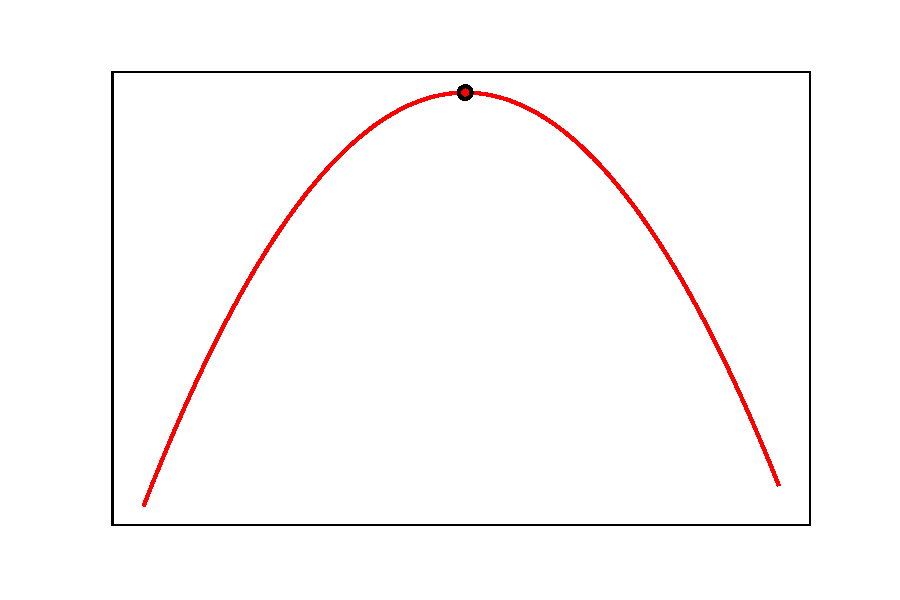
\includegraphics[width=\linewidth]{img/minimum}
		\caption{Ponto mínimo}
		\label{fig:minimo}
	\end{subfigure}
	\hfill
	\begin{subfigure}[h]{0.3\linewidth}
		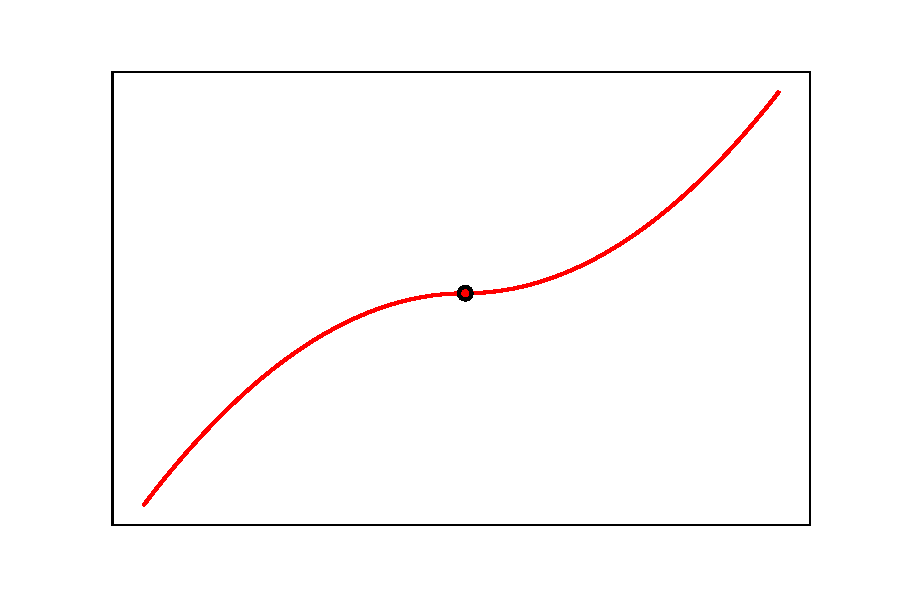
\includegraphics[width=\linewidth]{img/saddle}
		\caption{Ponto de sela}
		\label{fig:sela}
	\end{subfigure}%
	\caption{Exemplos de cada um dos três tipos de pontos críticos em funções no $R^2$}
	\label{fig:pontos_criticos}
\end{figure}

No contexto da otimização do desempenho resultante do ajuste de pesos de determinada RNA, a disparidade entre as saídas previstas $y_t$ e as saídas reais $y$ presentes no conjunto de dados deve ser minimizada. A função $y=f(x)$ que exprime a variância entre estes valores para um modelo de \emph{ML}, é comumente chamada de \emph{função custo}, e definida a partir da estimativa por máxima verossimilhança. Esta estimativa consiste de um método estatístico aplicado com o objetivo de minimizar a dissimilaridade entre a distribuição empírica $\hat{p}_{data}$ definida pelo conjunto de treinamento
e a distribuição do modelo.

A função custo utilizada por uma RNA é decomposta como uma soma de funções de perda aplicadas aos exemplos de treinamento. Uma das funções custo que podem ser utilizadas, descrita na Equação \ref{eq:custo}, consiste na probabilidade logarítmica condicional negativa dos dados de treinamento, onde $L$ é a perda calculada para cada exemplo dada na Equação \ref{eq:perda}.

\begin{equation}\label{eq:perda}
	L(x, y, \theta) = - \log p (y|x;\theta)
\end{equation}

\begin{equation}\label{eq:custo}
	J(\theta) = E_{x,y \sim \hat{p}_{data}} L(x, y, \theta) = \frac{1}{m} \sum_{i=1}^{m} L(x^{(i)}, y^{(i)}, \theta)
\end{equation}

Para estas funções custo, o gradiente descendente é computado através da Equação
\ref{eq:gradiente}. O custo operacional desta operação é $O(m)$, sendo $m$ o número de exemplos no conjunto de treinamento. Assim, o custo computacional cresce de maneira proporcional ao tamanho do conjunto de treinamento.

\begin{equation}\label{eq:gradiente}
	\nabla_{\theta} J(\theta) = \frac{1}{m} \sum_{i=1}^{m} \nabla_{\theta} L(x^{(i)}, y^{(i)}, \theta)
\end{equation}

A escolha da função de ativação está diretamente relacionada às escolhas de funções de ativação $g(z)$ de camadas ocultas e da camada de saída. Várias funções podem ser utilizadas, a depender do tipo de processamento e de saída desejada, contanto que sejam contínuas e deriváveis \cite{hornik1991approximation}. As funções de ativação mais comuns estão detalhadas na Tabela \ref{tab:ativacoes}.

%!TEX root = ../main.tex

\begin{table}[H]
	\scalefont{0.8}
	\centering
	\label{tab:ativacoes}
	\begin{adjustbox}{width=0.7\textwidth}
		\begin{tabular}{l l p{6.5cm} l}
			\toprule
			Nome 			 		& Gráfico & Equação & Intervalo\\
			\midrule
			Identidade ou Linear		&
			 	\Centerstack{\includegraphics[width=0.15\textwidth]{img/identidade}}
			&
				$
					\begin{aligned}
						\sigma(z) = z
					\end{aligned}
				$
				& $(-\infty, + \infty) $\\
			\hline
			Tangente Hiperbólica		&
				\Centerstack{\includegraphics[width=0.15\textwidth]{img/tanh}}
				&
				$
					\begin{aligned}
						\sigma(z) = tanh(z) =\frac{(e^z - e^{-z})}{(e^z + e^{-z})}
					\end{aligned}
				$
				 & $(-1,1)$\\
			\hline
			Sigmoide ou Logística		&
				\Centerstack{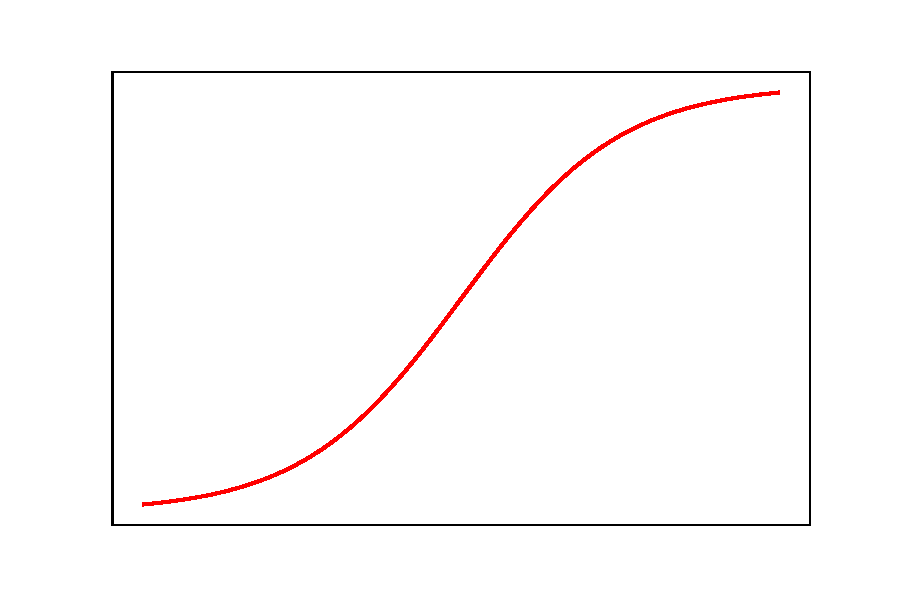
\includegraphics[width=0.15\textwidth]{img/sigmoid}}
				&
				$
					\begin{aligned}
						\sigma(z) = \frac{1}{1+e^{-x}}
					\end{aligned}
				$
				& $ (0,1) $\\
			\hline
			Unidade Linear Retificada	&
				\Centerstack{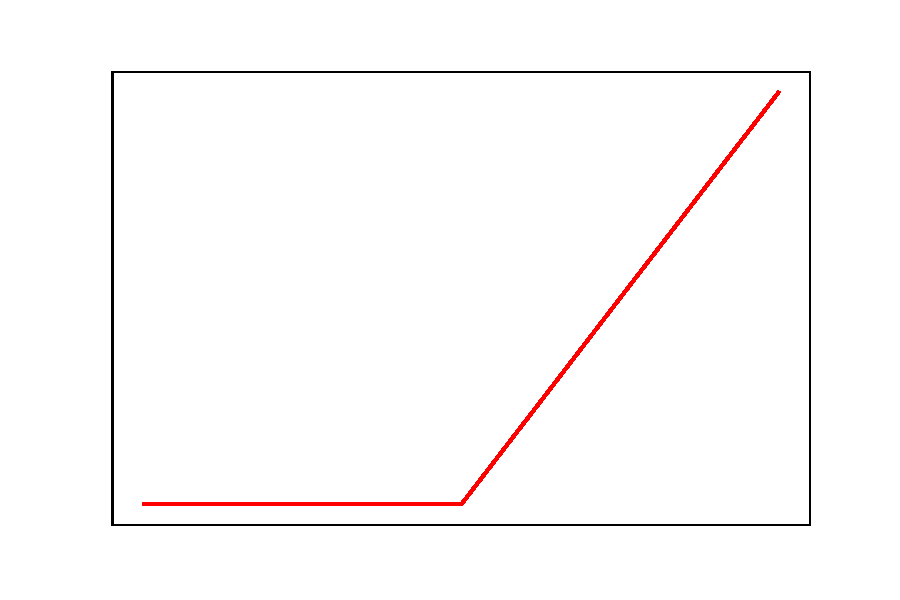
\includegraphics[width=0.15\textwidth]{img/relu}}
				&
				$
					\begin{aligned}
						\sigma(z) = max(0,z)
					\end{aligned}
				$
				& $ [0, \infty) $\\
			\hline
			Softmax					&
				\Centerstack{\includegraphics[width=0.15\textwidth]{img/softmax}}
				&
				$
					\begin{aligned}
						g(z_j) = \frac{e^{z_j}}{\sum^K_{j=1} e^{z_k}} \hspace{0.2cm}j=1, \ldots, K
					\end{aligned}
				$
				& $(-\infty, \infty)$\\
			\bottomrule
		\end{tabular}
	\end{adjustbox}
	\caption{Exemplos de funções de ativação}
\end{table}


As RNAs \emph{feedforward} formam a base para muitas aplicações. Inicialmente, este modelo era aplicado principalmente no mercado financeiro. Um exemplo desta utilização é o Sistema de Marketing Alvo, em inglês \emph{Target Marketing System}, utilizado nos anos 1990 pela \emph{Veratex Corp} para otimizar estratégias de marketing e cortar custos de marketing ao remover improváveis futuros consumidores de listas de compradores potenciais \cite{widrow1994neural}. Usos mais tardios também envolvem alocação de assentos em aviões, aprovação de empréstimo, controle de qualidade em processos industriais, entre outros. Quanto à detecção de padrões, destaca-se o uso de redes neurais convolucionais no reconhecimento de caracteres e dígitos escritos à mão, à exemplo de \cite{lenet}. Na medicina, algumas aplicações de RNA convolucionais, compreendidas na sub-área \emph{Deep Learning} (DL), podem compreender o aprimoramento e na segmentação de imagens cardíacas \cite{oktay2018anatomically}, aa classificação holistica de padrões de atenuação em tomografias computadorizadas para doenças do tecido intersticial do pulmão \cite{mingchen2018holistic}, e a leitura de mamografias computarizadas \cite{dubrovina2018mammography}. Atualmente, o modelo de RNA \emph{feedforward multilayer perceptron} tem grande destaque dentre as técnicas de ML. Estes modelos são parte da sub-área \emph{Deep Learning}, que será tratada na Seção \ref{sec:dl}.
